
\chapter{Design of Module \textit{threads}}

\section{Alarm clock}

    \subsection{Initial Functionality}

	At the beginning of this project the function \textit{sleep\_timer} is implemented as a busy wait. We want to reimplement it to avoid the busy wait.

    \subsection{Data Structures and Functions}

    \begin{lstlisting}
	struct thread
	{

	      ...
	  /* the time (in number of ticks) at which a 
	      sleeping thread should wake up */
	      int64_t wakeup_time;		
	      ...

	};
	
	/* a sorted list containing all sleeping 
	(blocked) threads. Sorting is done using 
	thread_wakeup_time_comparison function*/
	static struct list sleep_list;

	/* comparison function to order the sleeping
	threads ascending by their wakeup time */
	list_less_func thread_wakeup_time_comparison;

	/* sets the time at which the thread should 
	wake up and puts the thread in the sleeping 
	threads list */
	void thread_sleep (int64_t wakeup_time);

	/*this function checks if there are sleeping
	threads that should wake up at this moment 
	and calls the function thread_unblock for 
	each of those threads.*/
	void handle_sleeping_threads();    
    \end{lstlisting}


    \subsection{Functionality}

	When the function \textit{sleep\_timer} is called, this function calculates the time (in ticks) at which the thread should wake up, sets this time in the thread structure, inserts the thread in a sleeping list and then calls \textit{thread\_block}, in order to set the status THREAD\_BLOCKED, and to call the scheduler. The sleeping list is sorted ascending according to the time at which the threads should wake up (the first thread in this list is the thread that should wake up the earliest). At every timer interrupt, the function \textit{handle\_sleeping\_threads} is called which checks if there are threads that can wake up at the current moment of time. If there are, these threads are removed from the sleeping list, and \textit{thread\_unblock} is called on them, which sets their status to THREAD\_READY and puts them in the ready list.

	In order to avoid race conditions, the interrupts are disabled during the execution of \textit{sleep\_timer} and \textit{timer\_interrupt}.

    %\begin{figure}[h]
    %	\centering
    %	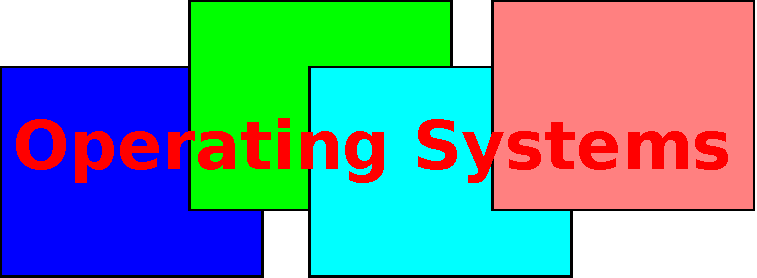
\includegraphics[width=0.5\textwidth]{figures/sample-image.pdf}
    %	\caption{Sample image}
    %	\label{fig:sample-image}
    %\end{figure}


    %Here you have a pseudo-code description of an algorithm taken fom \\ \href{http://en.wikibooks.org/wiki/LaTeX/Algorithms\_and\_Pseudocode\#Typesetting\_using\_the\_program\_package}{http://en.wikibooks.org/wiki/LaTeX}. It uses the \textit{program} package. Alternatively, you can use \textit{algorithmic} or \textit{algorithm2e} packages. 

    %\begin{program}
    %\mbox{Example of a pseudo-code algorithm description:}
    %\BEGIN %
    %  \FOR i:=1 \TO 10 \STEP 1 \DO
    %     |expt|(2,i); \\ |newline|() \OD %
    %\rcomment{This text will be set flush to the right margin}
    %\WHERE
    %\PROC |expt|(x,n) \BODY
    %          z:=1;
    %          \DO \IF n=0 \THEN \EXIT \FI;
    %             \DO \IF |odd|(n) \THEN \EXIT \FI;
    %\COMMENT{This is a comment statement};
    %                n:=n/2; x:=x*x \OD;
    %             \{ n>0 \};
    %             n:=n-1; z:=z*x \OD;
    %          |print|(z) \ENDPROC
    %\END
    %\end{program}


    \subsection{Design Decisions}

	This solution has the advantage that the time spent in the \textit{timer\_interrupt} function is constant, because the list is ordered. On the other hand the time spent for inserting is O(n), because we use a list to keep the threads. A better solution would be to use a heap as a data structure to keep the sleeping threads. In this way, the insertion timewould be only O(log n). 

	However, this solution is better than the solution in which at every \textit{timer\_interrupt} the whole sleeping list is traversed to see if there is a thread that should wake up even though the insertion is done in constant time, (without sorting the list) because \textit{timer\_interrupt} is called more often than the function \textit{sleep\_timer}.

    \subsection{Tests}

    alarm-single, alarm-multiple, alarm-negative, alarm-simultaneous, alarm-zero



\section{Priority scheduler}

    \subsection{Initial Functionality}

	At the beginning of this project the scheduler is implented as a Round-Robin scheduler. We want to reimplement it as a priority scheduler.

    \subsection{Data Structures and Functions}

    \begin{lstlisting}
      struct thread
      {
	    ...
	  /*the fixed priority of the thread,
	  given at creation */
	  int priority;
	  
	  /* the priority at a given moment of
	  the thread. This can be either the
	  thread's fixed priority or the 
	  priority inherited by donation */
	  int current_priority;		
	    ...
      };

      /* ready_list[i] contains the threads of
      priority i having the status THREAD_READY. */
      static struct list ready_list[PRI_MAX + 1];

      /* the priority scheduler */
      static struct thread * next_thread_to_run (void);

      /* promotes a thread to current thread's priority */
      void thread_promote (struct thread *);
      
      /* forces the current thread to return to it's
      default fixed priority. */
      void thread_lessen ();

      /* reimplementation of thread_unblock which checks 
      if the new READY thread is more prioritary than the 
      current thread, and if so, it forces current thread 
      to yield the cpu. */
      void thread_unblock (struct thread *);

      struct lock 
      {
	  struct thread *holder;   /* Thread holding lock */
	  unsigned value;          /* Current value. */
	  struct list waiters;     /* List of waiting threads. */
      };

      /* reimplementation of old lock functions according to
      the new structure of the lock */
      void lock_init (struct lock *);
      void lock_acquire (struct lock *);
      bool lock_held_by_current_thread (const struct lock *);

      /* reimplementation of old lock_acquire, with priority
      donation. When the lock is hold by a less prioritary
      thread, that thread is promoted to current thread's
      priority. */
      bool lock_try_acquire (struct lock *);

      /* reimplementation of old lock_release, with priority
      donation. If current thread was promoted, it gives up
      to it's inherited priority after releasing the lock. */
      void lock_release (struct lock *);      

    \end{lstlisting}


    \subsection{Functionality}

	The ready list is organized as a vector of lists, in which, every list contains threads that have the same priority. The scheduler calls the function \textit{next\_thread\_to\_run} which pops the most prioritary thread from its list and returns it; if there are more threads with the same priority, a round-robin algorithm is used. In order to avoid priority inversion, the \textit{lock\_aquire} is rewritten, so that whenever a thread with a greater priority waits for a lock holded by a thread with a lower priority, the function \textit{lock\_aquire} calls the function \textit{thread\_promote (holder)}. The function \textit{thread\_promote} sets the new current priority  for the holder to the priority of the current thread and then moves the thread in the ready lists vector from its list to the beginning of the list corresponding to its new priority. At the next call of the scheduler, the thread that holds the lock will receive cpu, and will be able to release the lock. In order to bring things back to previous situation, the function \textit{lock\_release} is rewritten, so that it calls the function \textit{thread\_lessen}, which forces the current thread to go back to its fixed priority, and to yield the cpu. At the call of \textit{thread\_yield} the next thread will put itself in the ready list corresponding to its previous priority. 

	To be able to give the cpu to a new more prioritary thread when it occurs, the \textit{thread\_unblock} function is rewritten to do this test, and force current thread to yield the cpu if necessary.

	In order to avoid race conditions, the interrupts are disabled during the execution of \textit{thread\_promote} and \textit{thread\_lessen}, and of course during the execution of functions where it was previously disabled.

    %\begin{figure}[h]
    %	\centering
    %	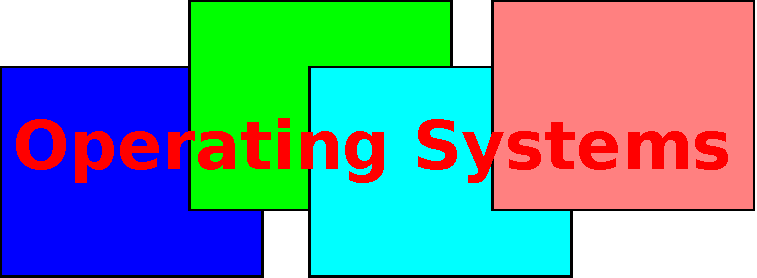
\includegraphics[width=0.5\textwidth]{figures/sample-image.pdf}
    %	\caption{Sample image}
    %	\label{fig:sample-image}
    %\end{figure}


    %Here you have a pseudo-code description of an algorithm taken fom \\ \href{http://en.wikibooks.org/wiki/LaTeX/Algorithms\_and\_Pseudocode\#Typesetting\_using\_the\_program\_package}{http://en.wikibooks.org/wiki/LaTeX}. It uses the \textit{program} package. Alternatively, you can use \textit{algorithmic} or \textit{algorithm2e} packages. 

    %\begin{program}
    %\mbox{Example of a pseudo-code algorithm description:}
    %\BEGIN %
    %  \FOR i:=1 \TO 10 \STEP 1 \DO
    %     |expt|(2,i); \\ |newline|() \OD %
    %\rcomment{This text will be set flush to the right margin}
    %\WHERE
    %\PROC |expt|(x,n) \BODY
    %          z:=1;
    %          \DO \IF n=0 \THEN \EXIT \FI;
    %             \DO \IF |odd|(n) \THEN \EXIT \FI;
    %\COMMENT{This is a comment statement};
    %                n:=n/2; x:=x*x \OD;
    %             \{ n>0 \};
    %             n:=n-1; z:=z*x \OD;
    %          |print|(z) \ENDPROC
    %\END
    %\end{program}


    \subsection{Design Decisions}

	why promoting/lessening is done in \textit{lock\_aquire} / \textit{lock\_release}?

	Another idea is to handle this in thread\_tick procedure, but we found out that it's generally a bad idea to load the interrupt handling code. If we would choose to do that the running time on each thread\_tick interrupt could degenerate to O(n) where n is the lock count of the system. So for each thread that is running and waiting for a lock to edit the lock holder's priority and let the schedule decide. This also solves the locking stack problem.
	
	why vector of lists?
O(1) insertion/removal. We could alternatively use sorted data structures.

    \subsection{Tests}

	alarm-priority, priority-change, priority-condvar, priority-donate-chain, priority-donate-lower, priority-donate-multiple, priority-donate-nest, priority-donate-one, priority-donate-sema, priority-fifo, priority-preempt, priority-sema

\section{Advanced scheduler}

    \subsection{Initial Functionality}

	At the beginning of this project the scheduler is implented as a priority scheduler. We want to reimplement it as an advanced scheduler(4.4BSD).

    \subsection{Data Structures and Functions}

    \begin{lstlisting}

      /* create new files fixed_point.c and fixed_point.h*/

      struct thread
      {
	    ...
	  /* */
	  int nice;
	  /* */
	  int64_t recent_cpu;
	    ...
      };

      /* load average of the whole system */
      int64_t load_avg;

      /* add the following header functions in the file
	fixed_point.h. These function represents operation
	between fixed-points and integer values. The 
	implementation of the files are in the file 
        fixed_point.c.*/
	int64_t fp_from_int(int n);
	int fp_to_int_rz(int64_t fp);
	int fp_to_int_rn(int64_t fp);
	int64_t fp_add(int64_t x, int64_t y);
	int64_t fp_subtract(int64_t x, int64_t y);
	int64_t fp_mult(int64_t x, int64_t y);
	int64_t fp_div(int64_t x, int64_t y);
	int64_t fp_int_add(int64_t x, int y);
	int64_t fp_int_subtract(int64_t x, int y);
	int64_t fp_int_mult(int64_t x, int y);
	int64_t fp_int_div(int64_t x, int y);

      /* modify the function timer_interrupt in which we
	we calculate for each the recent_cpu using the 
	function thread_for_each */
	void timer_interrupt();

      /* add a new function that recompute the new priority
	if the priority has changed than the thread is 
        pop from the thread and inserted again with the
        new priority */
	void thread_recompute_priority( struct thread );

    \end{lstlisting}


    \subsection{Functionality}

	\begin{program}
	\mbox{The timer\_interrupt function modification:}     
	\PROC |timer\_interrupt|() \BODY
		recent\_cpu[running\_thread]:=recent\_cpu[running\_thread] + 1;
		\IF TIMER\_FREQ \% TIMER\_TICKS \EQ 0 
		      \THEN thread\_for\_each(all\_threads\_list, thread\_recompute\_priority); 
		      \ELSE thread\_recompute\_priority(running\_thread);
		\FI;
	\END;
	\PROC |thread\_recompute\_priority|(thread) \BODY
		ready\_threads = count(ready\_list);
		\mbox{Use functions from fixed-point.h lib to compute the next expressions};
		load\_avg:= (59/60) * load\_avg + (1/60)*ready_threads; 
		recent\_cpu[thread]:= (2*load\_avg)/(2 * load\_avg + 1) + recent\_cpu[t] + nice[t];
		new\_priority:=clamp(PRI\_MAX - (recent\_cpu / 4) - (nice * 2));
		old\_priority:=priority[thread];
		\IF new\_priority != old\_priority
		      \THEN remove(ready\_list[old\_priority], thread.elem);
			    push\_back(ready\_list[new\_priority], thread.elem);
		\FI;
	\END;
	\end{program}
	We keep the vector V, of queues that we used when building the priority scheduler. V[i] represents the queue with priority i. By convention when the schedule is called, the next\_thread\_to\_run() procedure will remove the thread from the V[i].front() (where i represents the index with the highest priority) and will push it back in V[newPriority] in thread\_yield() proc and thread\_unblock().


	It is important that computations for recent\_cpu and load\_avg are done with functions from fixed\_point.h, because these two variables are real numbers.

	In order to be able to choose between the MLFQS scheduler and the Priority Scheduler when running the tests, the thread\_mlfqs flag is used. If this flag is set, the functions 
	\begin{itemize}
	  \item \textit{thread\_create} ignores the priority given as a parameter, and creates a thread with priority PRI\_DEFAULT,
	  \item \textit{thread\_set\_priority}, does not change the priority anymore
	  \item \textit{lock\_aquire} and \textit{lock\_release} don't do priority donation anymore
	\end{itemize}

    \subsection{Design Decisions}
We chose the vector of queues because of O(1) constant time retrieval and insertion. This means that the scheduler will run with the same speed regardless of the numbers of threads that are currently in the system. The choice of editing the functions thread\_yield(), thread\_unblock() and next\_thread\_to\_run() is good because all the synchronization mechanisms and sleeps already depend on them so we don't need to worry about how they are implemented.



    \subsection{Tests}
